\section{Blockchain Validators Set as a Shared Entity}\label{sec:validators}





\begin{figure*}[t]
  \begin{center}
    \begin{lstlisting}[language=Takamaka]
public interface Validators<V extends Validator> extends SharedEntity<V,Offer<V>> {

  @View BigInteger getStake(V validator);

  @FromContract @Payable
  void reward(String behaving, String misbehaving, BigInteger gasConsumed);
}

public abstract class AbstractValidators<V extends Validator>
    extends SimpleSharedEntity<V,Offer<V>> {

  public AbstractValidators(V validator, BigInteger power) {
    super(validator, power);
  }

  public void reward(String behaving, String misbehaving, BigInteger gasConsumed) { ... }
}

public class TendermintValidators extends AbstractValidators<TendermintED25519Validator> {

  public TendermintValidators(TendermintED25519validator validator, BigInteger power) {
    super(validator, power);
  }
}
    \end{lstlisting}
  \end{center}
  \caption{The shared entity of the validators set of a Hotmoka blockchain.}\label{fig:validators}
\end{figure*}

The Hotmoka blockchain is built over Tendermint~\cite{Kwon14}, a
generic engine for replicating an application over a network of nodes. In our case,
the application is an executor of smart contracts in Java, such as that in
Fig.~\ref{fig:simple_shared_entity}. Tendermint is based on a proof of stake
consensus, which means that a selected dynamic subset of the nodes is in charge of
validating the transactions and voting their acceptance. 
As we have said,
Hotmoka models validator nodes as \<Validator> objects, that are externally owned accounts
with an extra identifier. In the specific case of a Hotmoka blockchain built over Tendermint,
validators are \<TendermintED25519Validator> objects whose
identifier is derived from their ed25519 public key (see Fig.~\ref{fig:validator}).
This identifier is public information, reported in the blocks or easily eavesdropped.
Tendermint applications can implement their own
policy for rewarding or changing the validators' set dynamically.

\begin{figure*}[ht]
\centering
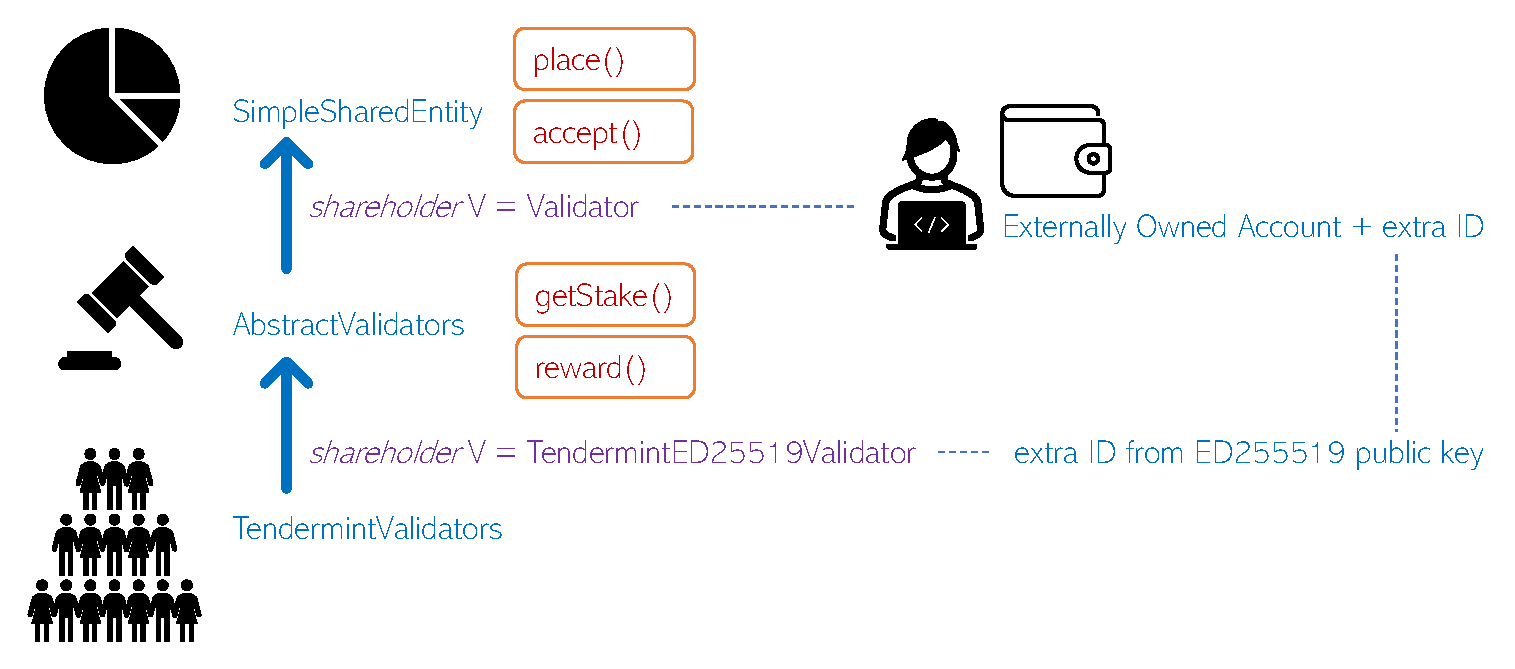
\includegraphics[width=0.8\linewidth]{figures/takamaka_validators}
\caption{Hierarchy of classes for implementing Hotmoka Validators.}
\label{figure.takamaka_validators}
\end{figure*}

The set of the validator nodes of a blockchain network is an example of a shared entity.
Namely, each such validator owns an amount of validation power, that corresponds to the shares
of a shareholder. Validation power can be sold and bought, exactly as shares.
Consequently, the \<Validators> interface in Fig.~\ref{fig:hierarchy-entities}
(reported in Fig.~\ref{fig:validators})
extends the \<SharedEntity> interface, fixes the shareholders to be
instances of \<Validator> and adds two methods: \<getStake> yields the money
at stake for each given validator (if the validator misbehaves, its stake will be reduced or
\emph{slashed}); and \<reward>, that is called by the blockchain itself at the end of each
block creation: it distributes the cost of the gas consumed by the transactions of the block,
to the well-behaving validators, and slashes the stakes of the misbehaving validators.

The \<AbstractValidators> class implements the validators' set
and the distribution of the reward and is a subclass of \<SimpleSharedEntity>
(see Fig.~\ref{fig:validators} and Fig.~\ref{figure.takamaka_validators}).
Shares are voting power in this case.
Its subclass \<TendermintValidators> restricts the type of the validators
to be \<TendermintED25519Validator>.
At each block committed, Hotmoka calls the \<reward> method of \<Validators>
in order to reward the validators that behaved correctly
and slash those that misbehaved, possibly removing them from the validators' set.
They are specified by two strings
that contain the identifiers of the validators, as provided by the underlying
Tendermint engine.

Since \<SimpleSharedEntity> allows shares to be sold and bought, this holds for
its \<TendermintValidators> subclass as well: the set of validators
is dynamic and it is possible to sell and buy voting power in order to invest in the blockchain
and earn rewards at each block committed. At block creation time,
Hotmoka calls method \<getShareholders> inherited from
\<SimpleSharedEntity> and informs the
underlying Tendermint engine about the identifiers of the validator nodes for the next blocks.
Tendermint expects such validators to mine and vote the subsequent blocks, until a change in the
validators' set occurs.

